% Created 2024-07-22 Mon 15:04
% Intended LaTeX compiler: pdflatex
\documentclass[letterpaper, 12pt]{article}
\usepackage[utf8]{inputenc}
\usepackage[T1]{fontenc}
\usepackage{graphicx}
\usepackage{longtable}
\usepackage{wrapfig}
\usepackage{rotating}
\usepackage[normalem]{ulem}
\usepackage{amsmath}
\usepackage{amssymb}
\usepackage{capt-of}
\usepackage{hyperref}
\usepackage{minted}
\usepackage{xcolor}
\usepackage{hyperref}
\usepackage{tocloft}
\usepackage{minted}
\usemintedstyle{manni}
\usepackage{pdfpages}
\usepackage{fancyhdr}
\usepackage{graphicx}
\usepackage[top=1.4in, left=0.5in, right=0.5in, bottom=0.8in]{geometry}
\usepackage[T1]{fontenc}
\usepackage{helvet}
\pagestyle{fancy}
\renewcommand{\headrulewidth}{0pt}
\renewcommand{\footrulewidth}{0pt}
\setlength{\parindent}{0em}
\setlength{\parskip}{1em}
\usepackage{hyperref}
\usepackage{color}
\hypersetup{
colorlinks=true,
linkcolor=blue,
filecolor=magenta,
urlcolor=cyan,
citecolor=green,
pdfborder={0 0 0}
}
\addtolength{\evensidemargin}{-2in}
\addtolength{\topmargin}{-0.5in}
\addtolength{\textwidth}{0in}
\usepackage[most]{tcolorbox}
\author{Hilduara Abreu}
\date{\today}
\title{Carta de Bienvenida 3K and PRE-K\\\medskip
\large llegadanuevo ano escolar 2024-25}
\hypersetup{
 pdfauthor={Hilduara Abreu},
 pdftitle={Carta de Bienvenida 3K and PRE-K},
 pdfkeywords={},
 pdfsubject={},
 pdfcreator={Emacs 29.3 (Org mode 9.8)}, 
 pdflang={English}}
\begin{document}

\fancyfoot[C]{\setlength{\unitlength}{1in}\begin{picture}(5,0)\put(-1.8,-1){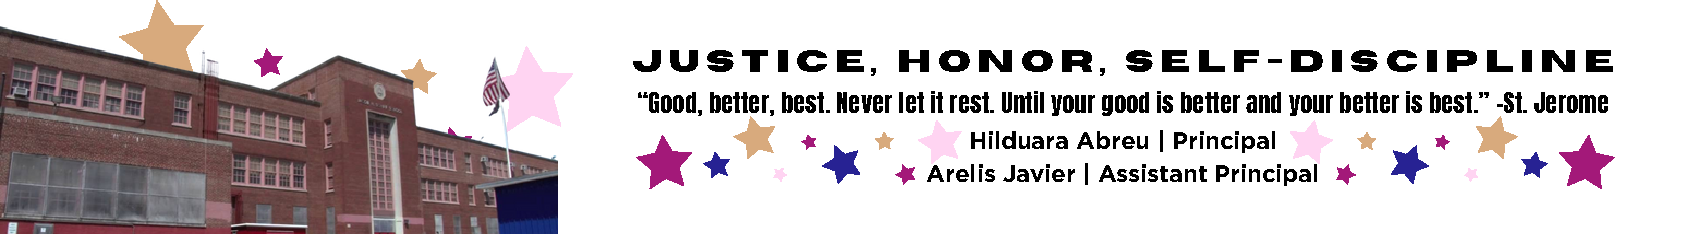
\includegraphics[width=8.8in,height=1.3in]{logo-1}}\end{picture}}
\fancyhead[C]{\setlength{\unitlength}{1in}\begin{picture}(5,0)\put(-1.9,-1){
\includegraphics[width=8.9in,height=1.3in]{logo-2}}\end{picture}}
\pagenumbering{gobble}
\usepackage{tcolorbox}
\newtcolorbox{redbox}[1][]{
  colback=red!5!white,
  colframe=red!75!black,
  fonttitle=\bfseries,
  coltitle=black,
  enhanced,
  attach boxed title to top center={yshift=-2mm},
  title=#1,
  boxed title style={colback=red!50!white}
}
\vspace*{0.3in}
\section*{Subject: Carta de Bienvenida | School Year: \href{https://www.ps192.org}{2024-25}}
\label{sec:orgbec1f9d}

Estimadas familias de 3-K y Pre-K,

¡Estamos emocionados contando los días hasta la llegada de nuestros estudiantes el jueves 5 de septiembre de 2024! Nuestros dedicados instructores y personal escolar esperan ansiosamente darles la bienvenida a lo que promete ser un emocionante año de fomentar conexiones y construir una sólida comunidad. Nuestros atentos educadores están emocionados por compartir su alegría, energía y pasión por el aprendizaje con sus hijos.

Mientras nos preparamos para el regreso de su hijo, queremos compartir información importante que está en vigor en la PS 192 para garantizar una experiencia de aprendizaje segura y placentera para todos. Por favor, tomen nota de las siguientes pautas:

\begin{redbox}[Pautas a seguir]
\begin{enumerate}
    \item \textbf{Uniformes:} Todos los estudiantes deben venir vestidos con su uniforme escolar todos los días, que sigue siendo el mismo: una camisa burdeos y pantalones o faldas azul marino.
    \item \textbf{Llegada y salida:} Para garantizar un proceso de llegada y salida seguro y eficiente, tomen nota del siguiente horario. Habrá miembros del personal y señales que guiarán a las familias durante la primera semana de clases.
    \begin{itemize}
        \item \textbf{Llegada:} Patio trasero a las 8:00 AM
        \item \textbf{Salida:} Patio trasero a las 2:15 PM
    \end{itemize}
\end{enumerate}
\end{redbox}

Primeros días de clases: Si bien todos los estudiantes tendrán un día escolar de 8:00 a 2:20 PM todos los días, los padres están invitados a quedarse con sus hijos el jueves y el viernes de 8:00 a 10:00 AM para ayudar a nuestros jóvenes estudiantes a adaptarse de manera más fluida al entorno escolar.

Suministros escolares: PS 192 proporcionará todos los suministros escolares básicos, como cuadernos, carpetas y crayones. Solo pedimos a las familias de 3K y PreK que proporcionen una mochila, ropa de cambio y suministros para su siesta diaria (manta, sábana y/o un pequeño objeto de transición como una muñeca o un peluche).

Nos sentimos privilegiados de ser parte de una comunidad donde padres, maestros, personal y estudiantes trabajan juntos para construir relaciones sólidas que respalden el crecimiento académico y social. Esperamos con ansias su participación en los diversos eventos a lo largo del año escolar y les damos la bienvenida a su participación activa en el viaje educativo de su hijo.

\pagebreak
\vspace*{0.4in}

Las actualizaciones regulares sobre eventos en toda la escuela se comunicarán a través de nuestro sitio web: \href{https://www.ps192.org}{www.ps192.org}, \href{https://www.classdojo.com/}{ClassDojo}, School Messenger y nuestro grupo de WhatsApp. Si tienen alguna pregunta, no duden en ponerse en contacto con nuestra Coordinadora de Padres, Angela Rijo, en \href{mailto:arijo@schools.nyc.gov}{arijo@schools.nyc.gov}, sitio web de la escuela: \href{https://www.ps192.org/angela}{www.ps192.org/angela}, o al (212) 775-9560.

Realizaremos eventos a lo largo del año y esperamos colaborar con ustedes tanto en persona como virtualmente. Manténganse atentos para obtener más información sobre todos nuestros próximos eventos:
\begin{itemize}
\item \textbf{El 12 de septiembre,} organizaremos nuestro primer Encuentro Virtual con el Maestro de su hijo de 4:30 PM a 7:30 PM
\end{itemize}

Estamos emocionados de comenzar este año escolar y de interactuar con ustedes para garantizar que su hijo disfrute de la mejor experiencia de aprendizaje posible, una en la que se sientan valorados, alentados y emocionados por aprender y sus infinitas posibilidades.

Es un honor profundo servir como directora de la PS 192. Gracias por su inquebrantable cooperación y dedicación a nuestros estudiantes, profesores y personal. Espero con ansias colaborar con ustedes en el viaje educativo de su hijo.

En unidad,


\includegraphics[width=100px,height=50px]{hil_signature.png}

\textbf{Hilduara Abreu}

\textbf{Principal}

\textit{The School of Joyful Learning!}

\href{https://www.ps192.org}{www.ps192.org}
\end{document}
